\chapter{\ifproject%
\ifenglish Project Structure and Methodology\else โครงสร้างและขั้นตอนการทำงาน\fi
\else%
\ifenglish Project Structure\else โครงสร้างของโครงงาน\fi
\fi
}

\enskip \enskip \enskip \enskip \enskip ในบทนี้จะกล่าวถึงการการออกแบบและฟีเจอร์ของแอพพลิเคชั่น นโยบายความเป็นส่วนตัวของผู้ใช้ User interface และการออกแบบฐานข้อมูลของแอพพลิเคชั่น



\makeatletter

% \renewcommand\section{\@startsection {section}{1}{\z@}%
%                                    {13.5ex \@plus -1ex \@minus -.2ex}%
%                                    {2.3ex \@plus.2ex}%
%                                    {\normalfont\large\bfseries}}

\makeatother
%\vspace{2ex}
% \titleformat{\section}{\normalfont\bfseries}{\thesection}{1em}{}
% \titlespacing*{\section}{0pt}{10ex}{0pt}

\section{โครงสร้างของแอพพลิเคชั่น}
\enskip \enskip \enskip \enskip \enskip 
แอปพลิเคชั่นนี้แบ่งออกเป็น ดังนี้ frontend
Backend hyperledger fabric blockchain และ database ซึ่งทำงานร่วนกัน
\subsection{Frontend}
\enskip \enskip \enskip \enskip \enskip 
เป็นส่วนแสดงผลหน้าจอของเว็บไซต์ เป็นส่วนที่เชื่อมต่อผู้ใช้กับ application โดยจะใช้ react ในการแสดงผล

\subsection{Hyperledger fabric Blockchain}
\enskip \enskip \enskip \enskip \enskip 
เป็นส่วนของPrivate blockchain ที่แอปพลิเคชั้นนี้ใช้เก็บ transaction log ที่เก็บข้อมูลที่มีการเปลี่ยนแปลงใน worldstate

\subsection{Backend}
\enskip \enskip \enskip \enskip \enskip 
เป็นส่วนประมวลผลของแอปพลิเคชั่น เป็นส่วนประมวลผลการทำงานคำสั่งต่างๆเป็นตัวกลางในการรับส่งข้อมูลระหว่าง frontend กับ database โดยจะใช้เป็น ภาษา javascript

\subsection{Database}
\enskip \enskip \enskip \enskip \enskip 
เป็นฐานข้อมูลที่ใช้เก็บข้อมูลในworldstate เพื่อนำข้อมูลไปประมวลผลโดยจะใช้เป็น mongoDB
% \begin{figure}
% \begin{center}
% \includegraphics{800px-Briny_Beach.jpg}
% \end{center}
% \caption[Poem]{The Walrus and the Carpenter}
% \label{fig:walrus}
% \end{figure}

% ~\cite{aiw}
\section{ฟีเจอร์ของแอปพลิเคชั่น}
\enskip \enskip \enskip \enskip \enskip
ในแอปพลิเคชั่นจะมีUser 3 แบบ คือ สถานศึกษา นักศึกษา บริษัทต่างๆ

\subsection{ฟีเจอร์ของ สถานศึกษา}
\enskip \enskip \enskip \enskip \enskip 
ฝั่งสถานศึกษา คือฝั่งของผู้ใช้ที่ต้องทำการส่งข้อมูลเข้า blockchain เพื่อไปอัพเดตช้อมูลใน worldstate และรับรองความถูกต้องของข้อมูล
โดยมีฟีเจอร์ในการทำงานโดยต่อไปนี้
\begin{enumerate}
  \item การลงทะเบียนและยืนยัน ฝั่งสถานศึกษาต้องลงทะเบียนกับทางระบบแล้วจะได้ตัว key เพื่อมาใช้ในการยืนยันตัวตน
  \item การจัดการข้อมูล สถานศึกษาสามารจัดการข้อมูลต่างๆเข้า blockchain ได้ เช่นการเพิ่มข้อมูล แก้ไขข้อมูล
  \end{enumerate}

\subsection{ฟีเจอร์ของ นักศึกษา}
\enskip \enskip \enskip \enskip \enskip 
ฝั่งนักศึกษาสามารถเข้ามาดูข้อมูลต่างๆของตัวเองได้และสามารถ export one time key ส่งให้บริษัทตรวจสอบข้อมูลของตนเองได้
โดยมีฟีเจอร์ในการทำงานโดยต่อไปนี้
\begin{enumerate}
  \item การดูข้อมูลของตน นักกศึกษาจะlogin เข้าไปด้วย key และสามารถตรวจสอบข้อมูลรายวิชาต่างๆ ที่ได้ลงทะเบียนไป และสามารตรวจสอบ transaction log ได้ ว่ามีบริษัทไหนได้เข้ามาดูบ้าง
  \item การ export public-key นักศึกษาสามาร export Key ของตัวเองและนำไปให้บริษัทที่อยากตรวจสอบความถูกต้องของตนเองเพื่อเพิ่มความน่าเชื่อถือ
  \end{enumerate}
\subsection{ฟีเจอร์ของ บริษัท}
\enskip \enskip \enskip \enskip \enskip 
ในฝั่งของบริษัทจะสามารถนำ key ของนักศึกษามาตรวจสอบข้อมูลในระบบได้
\begin{enumerate}
  \item ระบบลงทะเบียน ก่อนที่บริษัทจะเข้ามาดูข้อมูลของนักศึกษานั้นต้องลงทะเบียนยืนยันตัวตนกับระบบเสียก่อน
  \item การตรวจสอบข้อมูลของนักศึกษา บริษัทสามารถตรวจสอบข้อมูลของนักศึกษาที่ตนเองได้รับ key มา และสามารถตรวจสอบ transaction log เพื่อดูความน่าเชื่อถือของข้อมูลได้
  \end{enumerate}
\section{นโยบายความเป็นส่วนตัว}
\begin{enumerate}
  \item ข้อมูลของนักศึกษาต้องได้รับการยินยอมจากเจ้าตัวเสียก่อนถึงจะสามารถเปิดเผยได้
  \item การตรวจสอบข้อมูลของนักศึกษารั้นสามารตรวจสอบได้แค่ วิชาที่เรียนมา วัตถุประสงค์ของวิชานั้น และสามารถยืนยันได้ว่านักศึกษาจบจากมหาวิทยาลัยนั้นจริงๆ
  \end{enumerate}
\enskip \enskip \enskip \enskip \enskip 
เป็นส่วนแสดงผลหน้าจอของเว็บไซต์ เป็นส่วนที่เชื่อมต่อผู้ใช้กับ application


\section{ตัวอย่างการออกแบบ User Interface}
\enskip \enskip \enskip \enskip \enskip 
ออกแบบโดยใข้ Figma ซึ่งเป็นเครื่องมือสำหรับการออกแบบUser Interface ที่ได้รับความนิยมสูงสุดในปัจจุบัน

\graphicspath{ {./images/} }
\begin{figure}[htbp]
  \centering 
  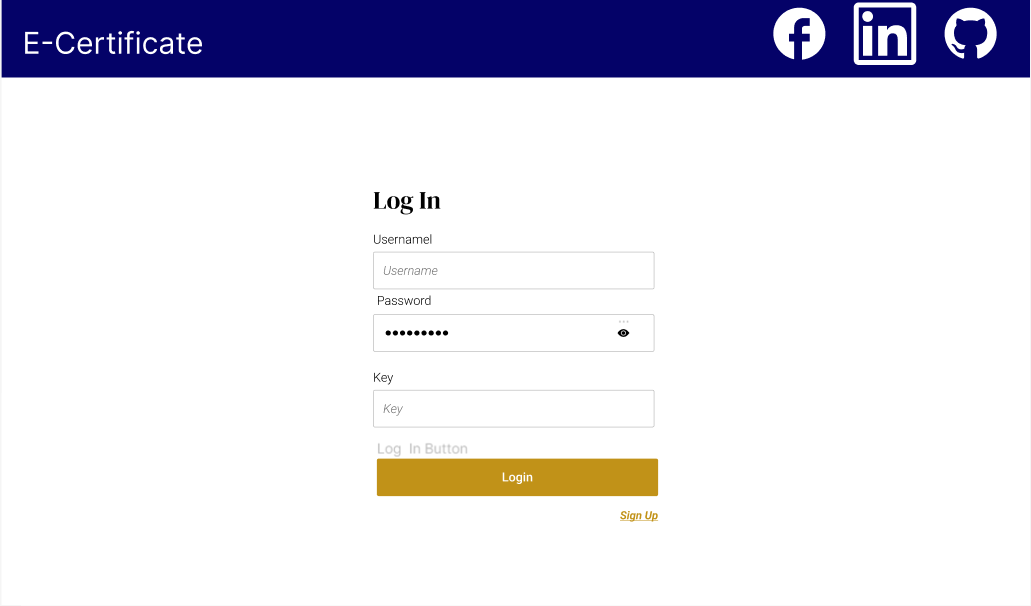
\includegraphics[scale=0.5]{figmalogin.png}
  \caption[หน้า Login]{หน้า Login}
  \label{fig:login}
\end{figure}

\graphicspath{ {./images/} }
\begin{figure}[htbp]
  \centering 
  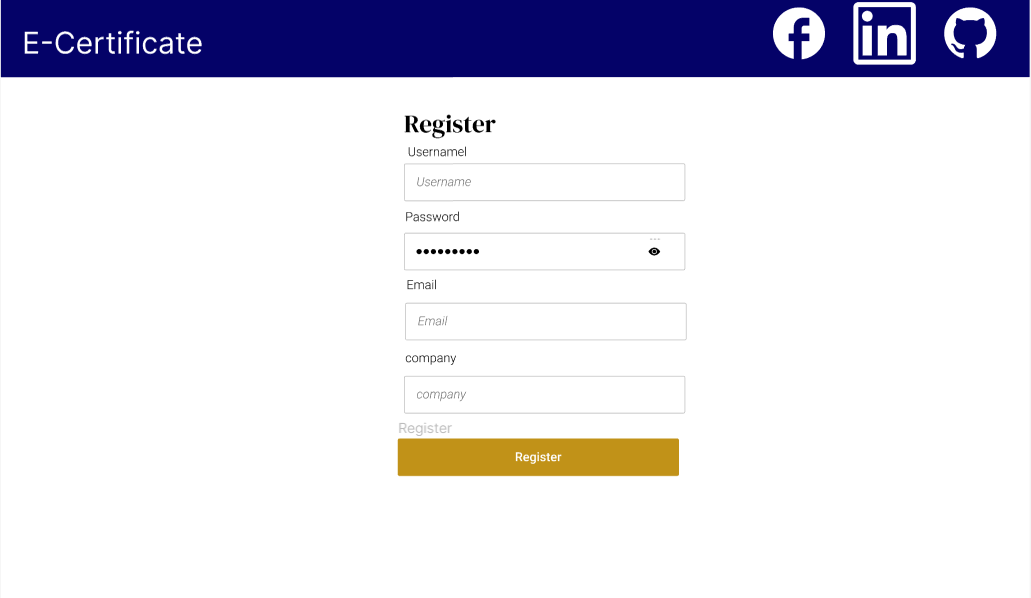
\includegraphics[scale=0.5]{figmaregis.png}
  \caption[หน้า Register]{หน้า Register}
  \label{fig:register}
\end{figure}

\graphicspath{ {./images/} }
\begin{figure}[htbp]
  \centering 
  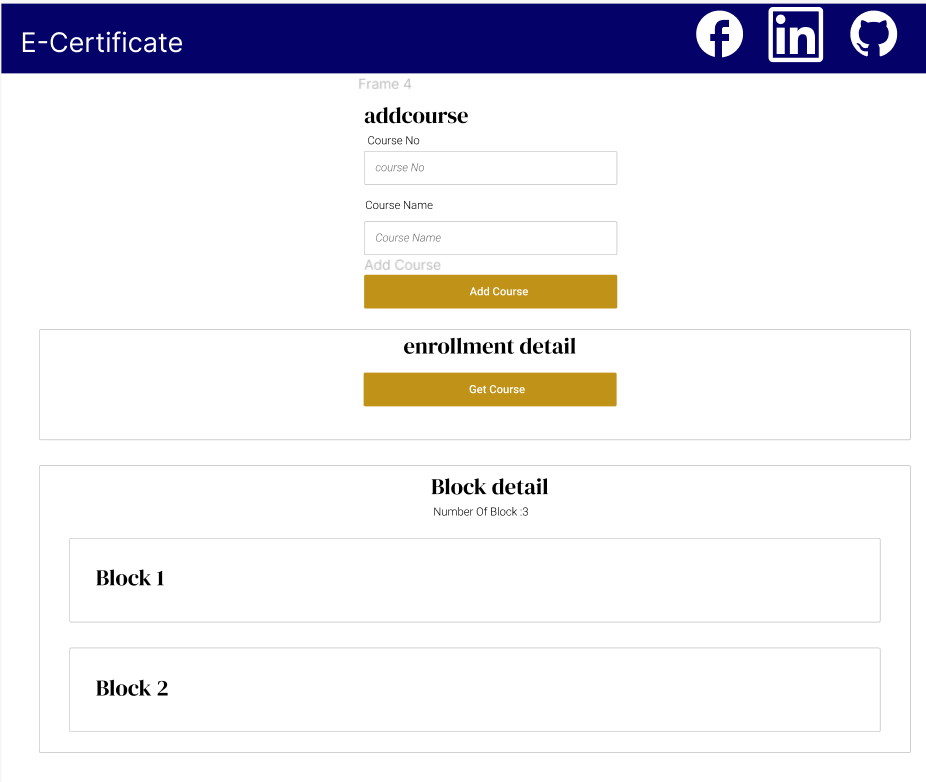
\includegraphics[scale=0.5]{figmaadd.png}
  \caption[หน้า Add course สำหรับสำนักทะเบียน]{หน้า Add course สำหรับสำนักทะเบียน}
  \label{fig:adding}
\end{figure}

\graphicspath{ {./images/} }
\begin{figure}[htbp]
  \centering 
  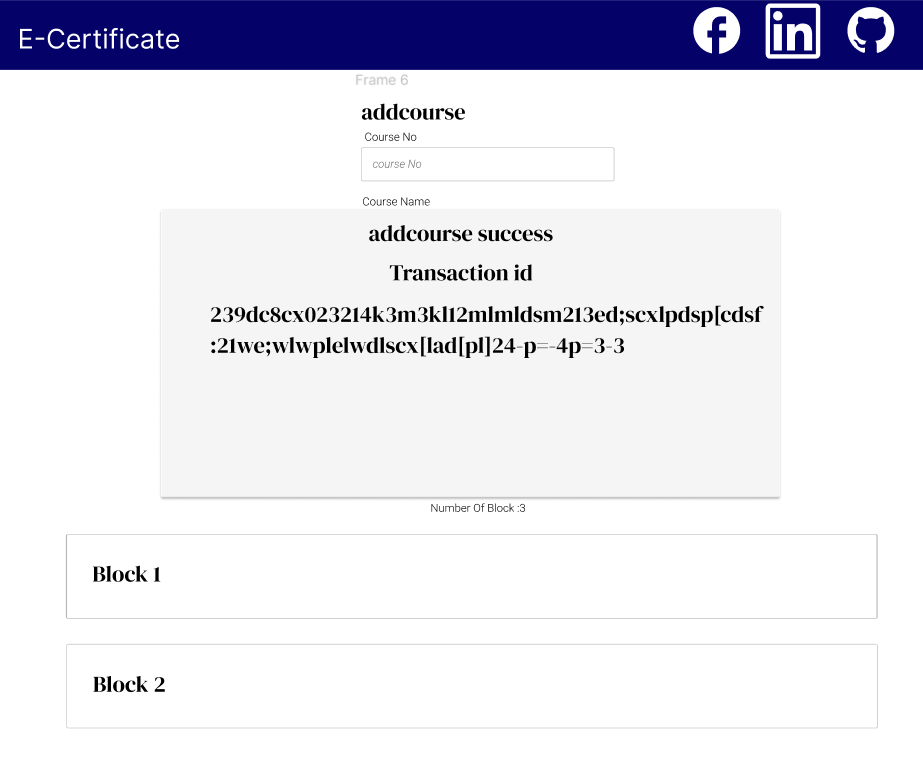
\includegraphics[scale=0.5]{addss.png}
  \caption[หน้า Add course Success]{หน้า Add course Success}
  \label{fig:add success}
\end{figure}

\graphicspath{ {./images/} }
\begin{figure}[htbp]
  \centering 
  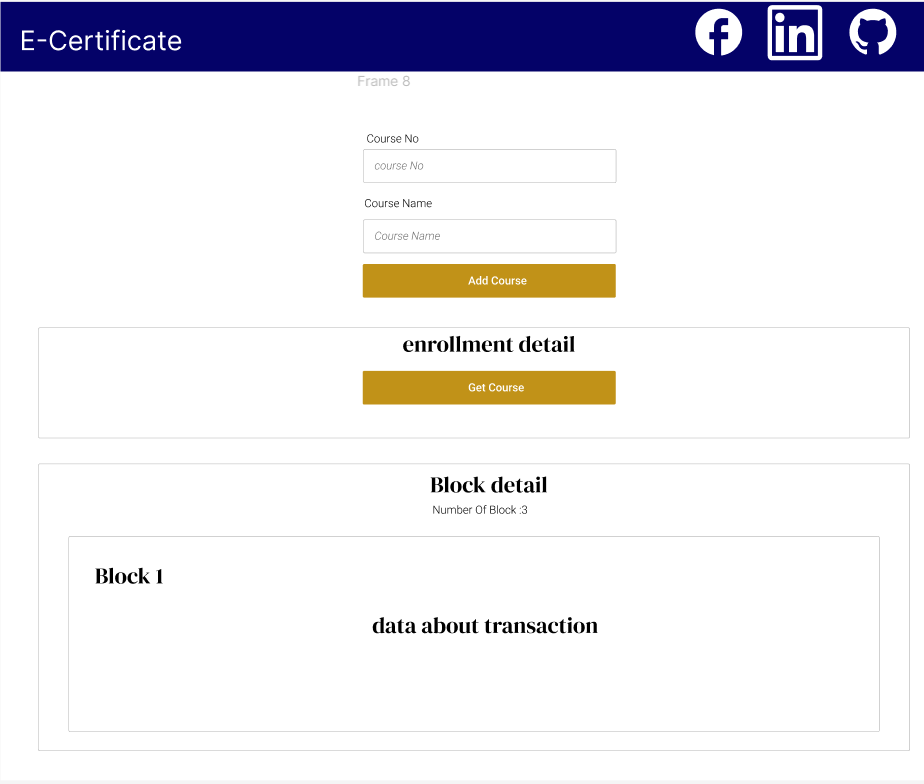
\includegraphics[scale=0.5]{blocktr.png}
  \caption[หน้าตรวจสอบ Transaction แต่ล่ะบล็อค]{หน้าตรวจสอบ Transaction แต่ล่ะบล็อค}
  \label{fig:block}
\end{figure}

\graphicspath{ {./images/} }
\begin{figure}[htbp]
  \centering 
  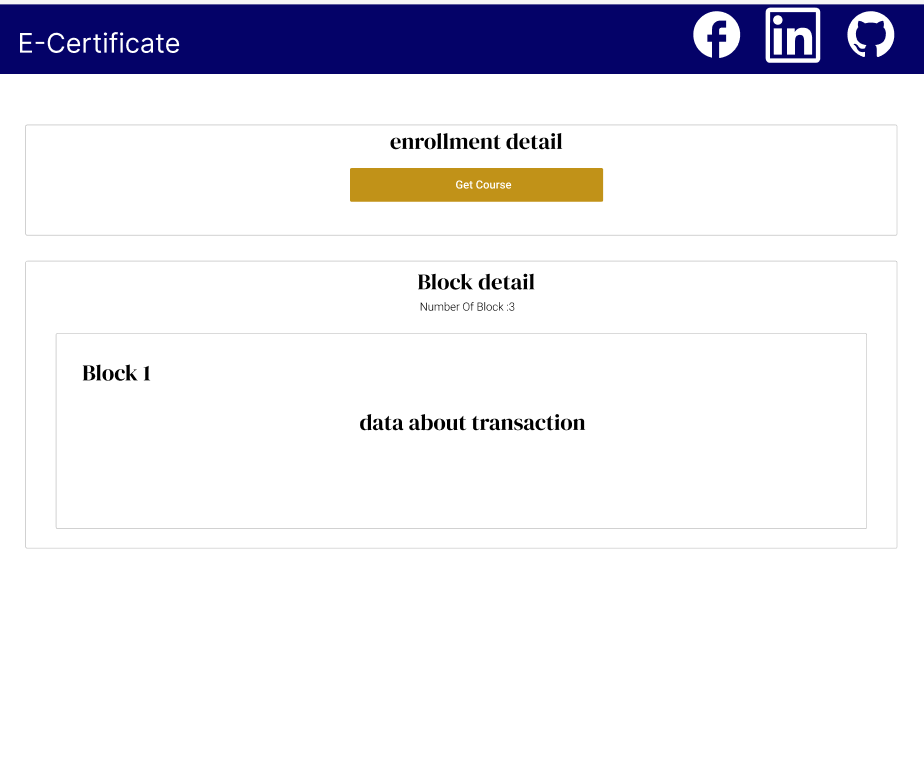
\includegraphics[scale=0.5]{company.png}
  \caption[หน้าหลังจากบริษัท login สำเร็จ]{หน้าหลังจากบริษัท login สำเร็จ}
  \label{fig:company}
\end{figure}

\graphicspath{ {./images/} }
\begin{figure}[htbp]
  \centering 
  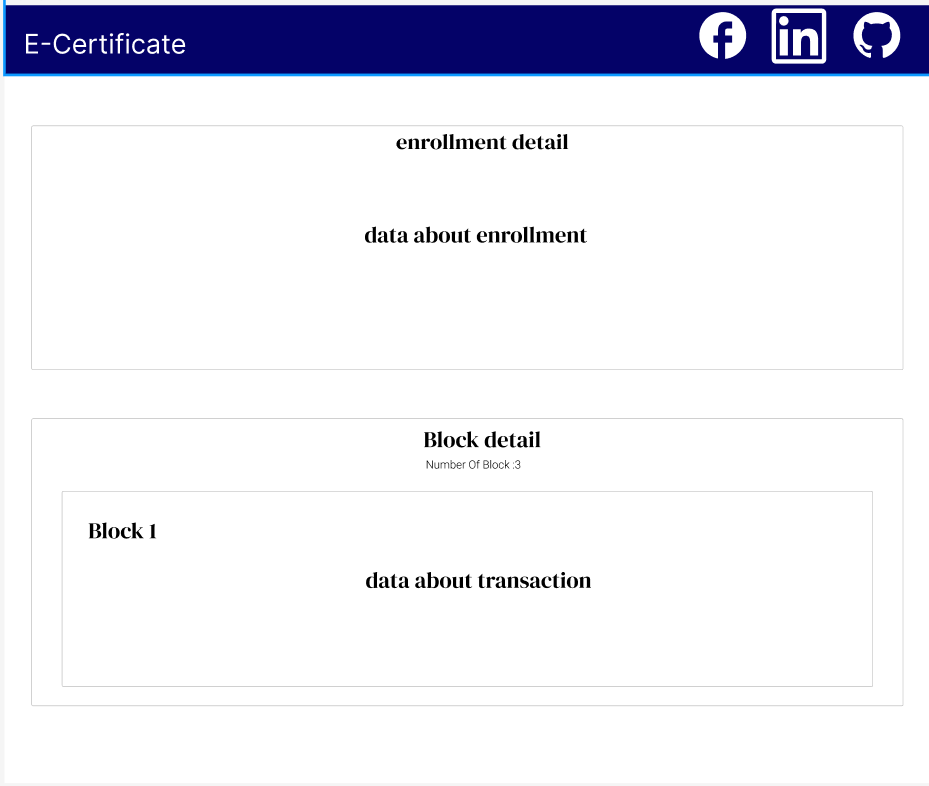
\includegraphics[scale=0.5]{comda.png}
  \caption[หน้าหลังจากบริษัท getข้อมูล]{หน้าหลังจากบริษัท getข้อมูล}
  \label{fig:getdata}
\end{figure}

\graphicspath{ {./images/} }
\begin{figure}[htbp]
  \centering 
  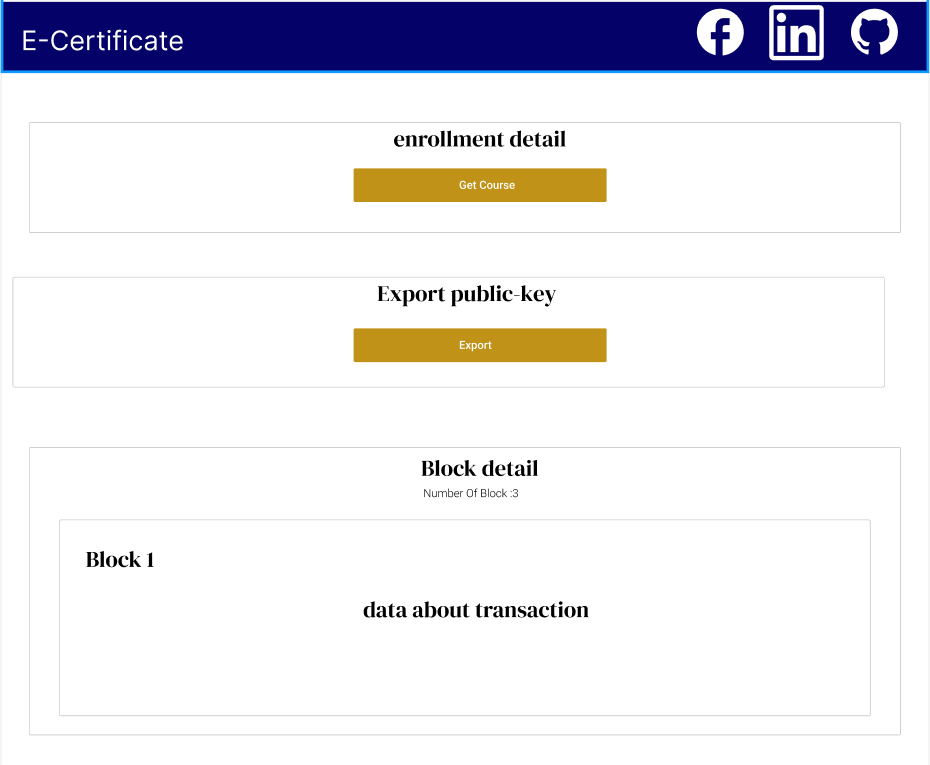
\includegraphics[scale=0.5]{st.png}
  \caption[หน้าหลังจากนักศึกษา login สำเร็จ]{หน้าหลังจากนักศึกษา login สำเร็จ}
  \label{fig:student}
\end{figure}


